%%%%%%%%%%%%%%%%%%%%%%%%%%%%%%%%%%%%%%%%%%%%%%%%%%%%%%%%%%%%%%%%%%%%%%%%
%    INSTITUTE OF PHYSICS PUBLISHING                                   %
%                                                                      %
%   `Preparing an article for publication in an Institute of Physics   %
%    Publishing journal using LaTeX'                                   %
%                                                                      %
%    LaTeX source code `ioplau2e.tex' used to generate `author         %
%    guidelines', the documentation explaining and demonstrating use   %
%    of the Institute of Physics Publishing LaTeX preprint files       %
%    `iopart.cls, iopart12.clo and iopart10.clo'.                      %
%                                                                      %
%    `ioplau2e.tex' itself uses LaTeX with `iopart.cls'                %
%                                                                      %
%%%%%%%%%%%%%%%%%%%%%%%%%%%%%%%%%%
%
%
% First we have a character check
%
% ! exclamation mark    " double quote  
% # hash                ` opening quote (grave)
% & ampersand           ' closing quote (acute)
% $ dollar              % percent       
% ( open parenthesis    ) close paren.  
% - hyphen              = equals sign
% | vertical bar        ~ tilde         
% @ at sign             _ underscore
% { open curly brace    } close curly   
% [ open square         ] close square bracket
% + plus sign           ; semi-colon    
% * asterisk            : colon
% < open angle bracket  > close angle   
% , comma               . full stop
% ? question mark       / forward slash 
% \ backslash           ^ circumflex
%
% ABCDEFGHIJKLMNOPQRSTUVWXYZ 
% abcdefghijklmnopqrstuvwxyz 
% 1234567890
%
%%%%%%%%%%%%%%%%%%%%%%%%%%%%%%%%%%%%%%%%%%%%%%%%%%%%%%%%%%%%%%%%%%%
%
\documentclass[10pt]{iopart}

\usepackage{citesort}

\usepackage{array}
\usepackage{textcomp}
\usepackage{graphicx}
\usepackage{stfloats}
\usepackage{float}
\usepackage{booktabs}
\usepackage{subcaption}
\usepackage{url}
%\usepackage{orcidlink}
\usepackage{pgfplots}
%\usepackage{hyperref}
\usepackage{tikz}
\usetikzlibrary{arrows.meta, positioning, shapes.geometric}
\newcommand{\gguide}{{\it Preparing graphics for IOP Publishing journals}}

\newcommand{\BibTeX}{Bib\TeX}
\newcommand{\REVTeX}{REV\TeX}

\sloppy 
%Uncomment next line if AMS fonts required
%\usepackage{iopams}  



\bibliographystyle{iopart-num}

\begin{document}

\title[Author guidelines for IOP Publishing journals in  \LaTeXe]
{Validation of a Theta/Alpha (Fz/Pz) EEG-Based Cognitive Load Index for Workload-Aware Human--Machine Systems}

\author{Edgar R. Hernandez-Rios$^1$$,^2$, 
Jerónimo Aparicio-Juarez$^1$, 
Omar A. Dominguez-Ramirez$^1$, 
Christian Penaloza$^2$$,^3$}

\address{$^1$ Universidad Autonoma del Estado de Hidalgo (UAEH), Pachuca, Mexico}
\address{$^2$ Mirai Innovation Research Institute, Osaka, Japan}
\address{$^3$ Universidad Autonoma de Chihuahua (UACH), Chihuahua, Mexico}

\ead{omar@uaeh.edu.mx}

\begin{abstract}

Workload-aware intelligent human--machine systems require reliable and interpretable user-state estimation mechanisms. This study validates an EEG-based cognitive load index defined as the ratio of frontal theta to parietal alpha power ($\theta_{Fz}/\alpha_{Pz}$) across two complementary paradigms: a controlled laboratory benchmark and an ecological interactive task.

In the controlled paradigm, passive reading (low demand) and Stroop interference (high demand) were used to manipulate workload. Six sessions satisfying predefined signal-quality criteria consistently exhibited higher $\theta_{Fz}/\alpha_{Pz}$ ratios during high demand, with group means increasing from 1.37 (SD = 1.80) to 4.65 (SD = 4.99) and a paired Cohen's $d=0.75$, supporting discriminative validity under well-defined conditions. In the ecological paradigm, the index was baseline-normalized during interactive task execution; 6 of 8 sessions showed increased ratios relative to baseline, indicating sensitivity to task engagement under realistic interaction variability.

NASA-TLX scores were collected to contextualize perceived workload. Overall, the results support the $\theta_{Fz}/\alpha_{Pz}$ ratio as a compact, interpretable, and implementation-ready metric for cognitive load estimation, suitable for integration into workload-aware human--machine systems.

\end{abstract}

%
% Uncomment for keywords
\vspace{2pc}
\noindent{\it Keywords}: EEG, Cognitive load estimation, Theta/Alpha ratio, User-state estimation, Workload-aware systems, Human--machine interaction, Neuroergonomics, Exergaming.
%
% Uncomment for Submitted to journal title message
%\submitto{\JPA}
%
% Uncomment if a separate title page is required
%\maketitle
% 
% For two-column output uncomment the next line and choose [10pt] rather than [12pt] in the \documentclass declaration
%\ioptwocol
%

%\keywords{magnetic moment, solar neutrinos, astrophysics}
%\submitto{\jpg}

\ioptwocol

\maketitle


\section{Introduction}

Quantifying cognitive load from neurophysiological signals is a central challenge in neuroergonomics, adaptive human--machine interaction, and intelligent training systems. Reliable estimation of cognitive workload enables the characterization of how task demands influence attention, executive control, and performance, and constitutes a key component for the development of systems capable of adapting to the user’s cognitive state \cite{24}. In domains such as robotics, immersive virtual environments, and interactive training platforms, real-time awareness of user workload has the potential to improve safety, optimize task difficulty, and maintain effective interaction between humans and intelligent systems.

Maintaining cognitive workload within an optimal range is particularly important for human performance. According to the classical Yerkes--Dodson relationship, both insufficient cognitive engagement (underload) and excessive mental demand (overload) can negatively affect performance. Systems capable of monitoring user workload in real time therefore enable adaptive strategies such as dynamic task difficulty adjustment, intelligent assistance, or workload-aware feedback. In this context, reliable and interpretable workload indicators are essential for maintaining users within an optimal cognitive operating range during interaction.

Among available sensing modalities, electroencephalography (EEG) has become one of the most widely used techniques for cognitive workload monitoring due to its high temporal resolution and its direct relationship with cortical processes underlying mental effort and attentional control. Numerous studies have demonstrated that specific spectral modulations in EEG activity are associated with variations in cognitive demand. In particular, increases in frontal theta activity (4--7~Hz) have been linked to executive control, conflict monitoring, and sustained attention, whereas decreases in parietal alpha activity (8--12~Hz) are commonly interpreted as markers of increased cortical engagement and information processing demand \cite{c8}. These spectral dynamics have been widely reported as robust EEG correlates of cognitive workload across experimental paradigms \cite{c1,c4}.

Frontal-midline theta activity has been specifically associated with cognitive control processes such as conflict monitoring and error processing, and is widely recognized as one of the most reliable spectral markers of mental effort \cite{CavanaghFrank2014_FrontalTheta}. In contrast, task-related alpha desynchronization—often prominent over posterior and parietal regions—reflects increased cortical engagement and active information processing due to a release of functional inhibition \cite{Klimesch2007_AlphaInhibitionTiming}. These complementary oscillatory dynamics provide a neurophysiological basis for constructing compact spectral indices capable of capturing variations in cognitive load.

Building on these findings, several studies have proposed ratio-based EEG metrics that combine theta and alpha activity into a single scalar indicator of cognitive load. Such ratios integrate complementary neural mechanisms—frontal executive engagement and parietal task-related desynchronization—while reducing feature dimensionality compared to multi-feature machine learning approaches. As a result, theta-to-alpha or alpha-to-theta ratios have been suggested as interpretable and computationally efficient workload indicators suitable for real-time monitoring in interactive systems \cite{c1,c7}. However, recent work emphasizes that the reliability and generalizability of EEG-based workload metrics depend strongly on methodological factors such as electrode configuration, preprocessing pipelines, artifact handling, and task context \cite{c4,c6,Mastropietro2023_ReliabilityFzPz}.

Despite the growing number of EEG-based workload metrics proposed in the literature, several methodological challenges remain. First, many studies rely on complex feature sets or machine learning models that are difficult to interpret and reproduce across laboratories. Second, validation is frequently performed only under tightly controlled experimental conditions, limiting the applicability of these approaches in real interactive environments. Third, differences in preprocessing pipelines, artifact rejection strategies, and electrode selection often make it difficult to compare results across studies. Standardized EEG preprocessing approaches have therefore been proposed to improve reproducibility and cross-study comparability \cite{BigdelyShamlo2015_PREP}. These challenges highlight the need for compact, interpretable workload indices validated through transparent processing pipelines and tested across both controlled and ecological task contexts.

Controlled cognitive interference paradigms, such as the Stroop task, are widely used as benchmarks for eliciting well-characterized increases in cognitive load. EEG studies consistently report increased frontal theta activity and modulation of alpha rhythms during Stroop interference, reflecting elevated executive and attentional demands \cite{c5,c9}. While these paradigms provide well-defined conditions for validating workload indices, many real-world human--machine systems operate in interactive environments where cognitive demand fluctuates dynamically and cannot be reduced to strictly scripted stimuli. Recent neuroergonomics studies demonstrate that EEG-based workload measures can also be observed in ecological tasks such as driving or real-flight monitoring, highlighting the importance of evaluating workload metrics under naturalistic interaction scenarios \cite{DiFlumeri2018_RealDrivingMWL,Dehais2019_RealFlightDryEEG}.

Despite substantial progress in EEG-based cognitive workload estimation, an important gap remains between laboratory validation and real-world deployment. Many proposed workload metrics rely on complex feature sets or machine learning models that limit interpretability and reproducibility across studies. At the same time, validation is frequently restricted to tightly controlled experimental paradigms, leaving open the question of whether the same indices remain sensitive under ecological interaction conditions where cognitive demand emerges dynamically during continuous tasks. Bridging this gap requires compact and neurophysiologically interpretable EEG metrics that can be validated using standardized processing pipelines and evaluated across both controlled cognitive paradigms and interactive task environments.

In this work, we investigate a compact EEG-based cognitive load index defined as the ratio of frontal theta power at Fz to parietal alpha power at Pz. This index combines two well-established spectral correlates of cognitive workload—frontal theta associated with executive control and parietal alpha desynchronization associated with increased cortical engagement—into a single interpretable metric. 
Figure~\ref{fig:study_overview} summarizes the conceptual framework of the study, illustrating how the controlled and ecological paradigms converge on a compact EEG-derived cognitive load index for validation across interaction contexts.

\begin{figure*}[t]\centering
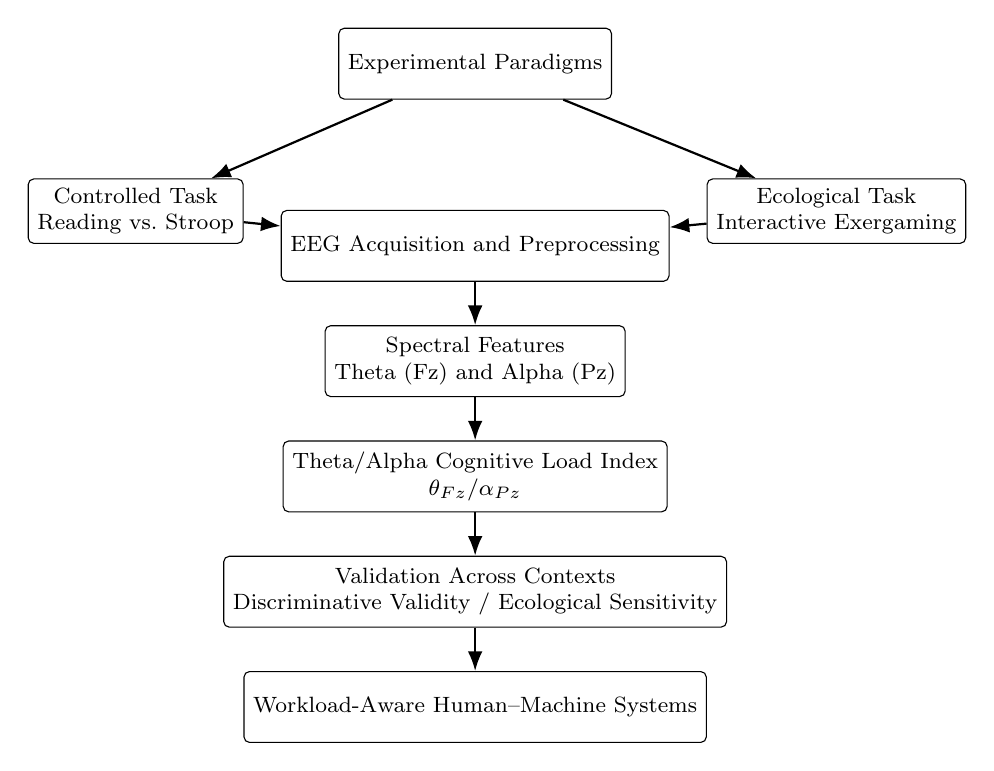
\begin{tikzpicture}[
    node distance=0.55cm and 0.9cm,
    every node/.style={font=\footnotesize, align=center},
    box/.style={
        draw,
        rounded corners=2pt,
        minimum width=2.9cm,
        minimum height=0.9cm,
        text centered
    },
    smallbox/.style={
        draw,
        rounded corners=2pt,
        minimum width=2.7cm,
        minimum height=0.8cm,
        text centered
    },
    arrow/.style={
        -{Latex[length=2.5mm]},
        thick
    }
]

\node[box] (paradigms) {Experimental Paradigms};

\node[smallbox, below left=1cm and 1.2cm of paradigms] (controlled)
{Controlled Task\\Reading vs.\ Stroop};

\node[smallbox, below right=1cm and 1.2cm of paradigms] (ecological)
{Ecological Task\\Interactive Exergaming};

\node[box, below=1.4cm of paradigms] (eeg) {EEG Acquisition and Preprocessing};

\node[box, below=of eeg] (features) {Spectral Features\\Theta (Fz) and Alpha (Pz)};

\node[box, below=of features] (index) {Theta/Alpha Cognitive Load Index\\$\theta_{Fz}/\alpha_{Pz}$};

\node[box, below=of index] (validation) {Validation Across Contexts\\Discriminative Validity / Ecological Sensitivity};

\node[box, below=of validation] (application) {Workload-Aware Human--Machine Systems};

\draw[arrow] (paradigms) -- (controlled);
\draw[arrow] (paradigms) -- (ecological);

\draw[arrow] (controlled) -- (eeg);
\draw[arrow] (ecological) -- (eeg);

\draw[arrow] (eeg) -- (features);
\draw[arrow] (features) -- (index);
\draw[arrow] (index) -- (validation);
\draw[arrow] (validation) -- (application);

\end{tikzpicture}
\caption{Conceptual overview of the study design. Two complementary paradigms—a controlled laboratory task and an ecological interactive task—are used to evaluate a compact EEG-based cognitive load index derived from frontal theta and parietal alpha activity.}
\label{fig:study_overview}
\end{figure*}

The main contributions of this work are threefold. First, we provide controlled validation of the $\theta_{Fz}/\alpha_{Pz}$ ratio using a classical cognitive interference paradigm (reading versus Stroop) together with predefined signal-quality criteria and session-level effect size estimation. Second, we evaluate the sensitivity of the same index under ecological interaction conditions using an interactive exergaming task involving sustained attention and sensorimotor coordination. Third, we present a transparent and reproducible EEG processing pipeline—including preprocessing, artifact handling, and spectral estimation—that supports the integration of compact workload indices into workload-aware human--machine systems.

%%%%%%%%%%%%%%%%%%%%%%%%%%%%%%%%%%%%%%%%%%%%%%%%%%%%%%%%%%%%%%%%%%%%%

\section{Interactive Exergaming Platform and Task Context}

To complement controlled laboratory benchmarks and examine the behavior of the proposed EEG-based cognitive load index under more ecological conditions, an interactive exergaming platform was employed as the task context for the ecological paradigm. Exergaming tasks provide structured yet flexible environments in which cognitive demand emerges from sustained attention, sensorimotor coordination, and continuous interaction, rather than from strictly scripted or time-locked stimuli. Prior work has used exergaming settings as interactive contexts where attention and engagement can be modulated by task demands~\cite{14,15}.

The exergaming environment used in this study, referred to as \emph{K9 Canine Quest}, was developed at the Advanced Robotics and Haptic Interfaces Laboratory (UAEH) as a modular interactive system integrating virtual environments, multiple input modalities, and force-feedback interaction~\cite{16}. While the platform has been explored in broader research contexts, in the present work it is used solely as an experimental task environment (not as a therapeutic or clinical intervention) to assess EEG-based cognitive load sensitivity under ecological and interactive variability. The inclusion of haptic interaction is motivated by prior research showing that force-feedback interfaces provide controlled sensorimotor interaction and reproducible coupling between user motion and virtual task dynamics~\cite{22,23}.

The task is implemented within a virtual environment that requires users to navigate, explore, and interact with on-screen elements while maintaining attention and responding to dynamic feedback. Cognitive demand arises from the coordination of perception, decision-making, and motor actions over sustained periods of interaction. Unlike controlled laboratory tasks, the exergaming scenario allows natural variability in user strategies, pacing, and engagement, providing a realistic context for evaluating the sensitivity of EEG-derived workload indices.


\begin{figure}[htbp]
\centering

\begin{subfigure}[t]{0.4\textwidth}
    \centering
    
\includegraphics[width=\linewidth]{figures/CQuest1.jpg}
    \caption{Virtual environment used for interactive task execution.}
\end{subfigure}
%\hfill
\medskip

\begin{subfigure}[t]{0.4\textwidth}
    \centering
    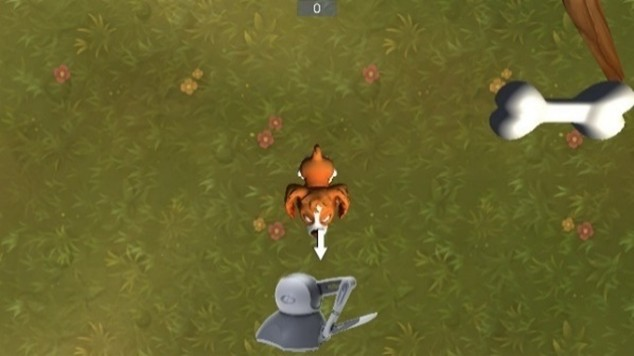
\includegraphics[width=\linewidth]{figures/CQuest2.jpg}
    \caption{Haptic interface enabling force-feedback interaction.}
\end{subfigure}

\medskip

\begin{subfigure}[t]{0.4\textwidth}
    \centering
    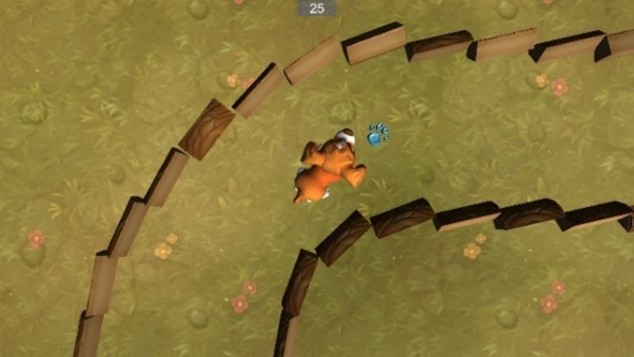
\includegraphics[width=\linewidth]{figures/CQuest4.jpg}
    \caption{User interaction during the exergaming task.}
\end{subfigure}

\caption{K9 Canine Quest exergaming platform used as an ecological interactive task context.}

\end{figure}

Multiple interaction modalities are supported by the platform, including keyboard, gamepad, and haptic interface control. These modalities enable different sensorimotor interaction styles while preserving a common task structure. In this study, interaction modality is treated as part of the ecological variability of the task rather than as an independent experimental factor, and analyses are conducted at the session level.

\subsection{Contextual Relevance of Neurophysiological Workload Monitoring}

Neurophysiological workload monitoring has been proposed as a means of characterizing cognitive demand in interactive systems, particularly in environments where task demands fluctuate dynamically~\cite{c10}. In EEG-based contexts, such monitoring can provide objective indicators of user state without relying solely on task performance or self-report measures.

In the present work, neurophysiological signals are not used to implement closed-loop adaptation, biofeedback, or therapeutic intervention. Instead, this perspective motivates the selection of an interactive task environment in which cognitive load naturally varies and can be quantified using EEG-derived indices. The exergaming platform therefore serves as a representative scenario for studying workload dynamics under ecological interaction conditions.

\subsection{Haptic Interaction in the Exergaming Task}

The haptic interface consists of an articulated-link mechanism designed to deliver tactile and kinesthetic feedback by engaging cutaneous mechanoreceptors, proprioceptors, and kinesthetic pathways. It enables bidirectional interaction with virtual environments through controlled force rendering, supporting immersive sensorimotor interaction during task execution~\cite{22,23}.

The system supports two general interaction modes: active haptic exploration and passive haptic guidance. In active exploration, users voluntarily control their movements to interact with the virtual environment, promoting sensorimotor engagement and exploratory behavior. In passive guidance, an external agent constrains or guides user motion during interaction. In the context of this study, these modes are considered interaction mechanisms that shape task engagement and cognitive demand, without implying therapeutic use or performance enhancement.


% \begin{figure*}[htbp]
%    \centering
%    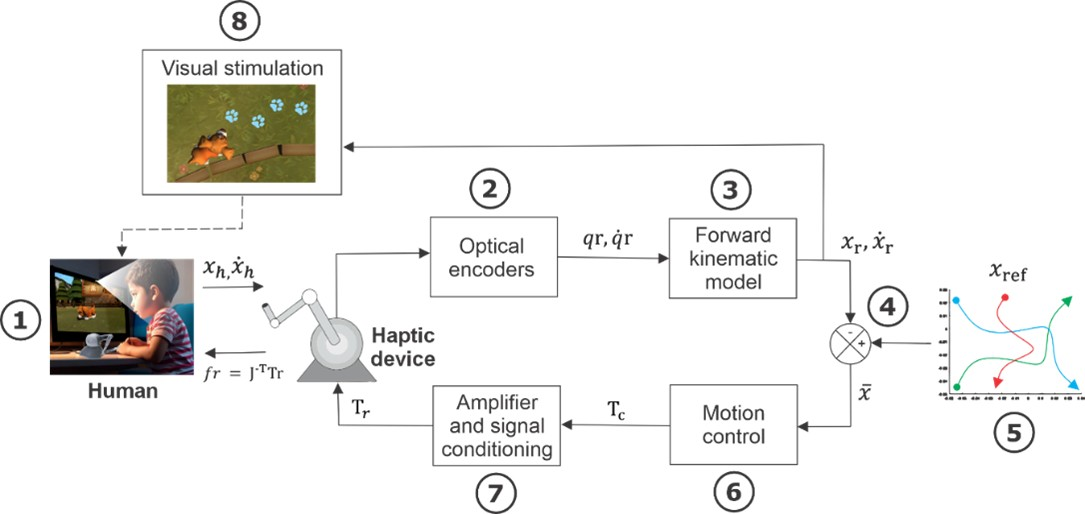
\includegraphics[width=1\linewidth]{figures/CQuest3.jpg}
%    \caption{Passive haptic guidance scheme within the exergaming interaction context.}
%    \label{CQuest3}
% \end{figure*}

\subsection{Role of the exergaming platform in cognitive load assessment}
Within this study, the exergaming platform serves as an ecological task context for examining the robustness and sensitivity of the EEG-based theta/alpha (Fz/Pz) index beyond controlled laboratory benchmarks. The platform introduces realistic sources of variability, including movement-related artifacts, fluctuating attention, and individual interaction strategies, which are characteristic of real-world human--machine interaction scenarios.

Accordingly, the exergaming task is not evaluated in terms of efficacy, training outcomes, or clinical impact. Rather, it is used as a representative interactive scenario in which cognitive load naturally emerges and can be quantified using neurophysiological indices.


%%%%%%%%%%%%%%%%%%%%%%%%%%%%%%%%

\section{Methods}

\subsection{Participants and data overview}
EEG was collected in a controlled protocol (14 sessions; 6 includable) and an ecological exergaming task (8 sessions). Analyses were session-level (some participants contributed multiple sessions). All participants provided informed consent under institutional procedures.

\subsection{EEG acquisition hardware and software}
EEG was recorded using the AURA device, an 8-channel EEG system with a nominal sampling rate of 250~Hz. Signals were streamed in real time using Lab Streaming Layer (LSL). A custom graphical interface implemented in PyQt5 was used to guide the experimental protocols and store recorded data as CSV files. Electrodes were positioned according to the international 10--20 system at Fp1, Fp2, F3, Fz, F4, P3, Pz, and P4, covering bilateral frontopolar, frontal, and parietal regions as well as the midline. The cognitive load index was computed using theta-band activity from Fz and alpha-band activity from Pz, selected based on prior evidence linking frontal theta and parietal alpha dynamics to cognitive workload.

\subsection{Offline preprocessing}
All EEG data were processed offline using a standardized preprocessing pipeline. Signals were notch filtered at 60~Hz (Q~=~30) to attenuate power line interference, followed by bandpass filtering between 1 and 40~Hz using a fourth-order Butterworth filter.

Common average reference (CAR) was applied in the ecological paradigm to improve robustness under movement-related noise inherent to interactive tasks. For the controlled paradigm, data were analyzed using the original reference configuration to preserve comparability with the acquisition setup and minimize additional signal transformations.

The effective sampling rate was assumed to be 250~Hz and was verified when necessary using signal timestamps.

\subsection{Spectral analysis and Cognitive Load Index (CLI)}
Spectral power was estimated using Welch’s power spectral density (PSD) method. EEG signals were segmented into windows of 250 samples (1~s at 250~Hz) with 50\% overlap (step size of 125 samples). For each window, theta-band power (4--7~Hz) was computed from channel Fz, and alpha-band power (8--12~Hz) from channel Pz. Bandpower was defined as the integral of the PSD over the corresponding frequency band using the trapezoidal rule.

The cognitive load index was defined for each window as:

\begin{equation}
\mathrm{Index} = \frac{\theta_{Fz}}{\alpha_{Pz}}.
\label{CLI2}
\end{equation}

Non-finite values were discarded and division by zero was avoided. Index values were averaged across valid windows within each phase or session.

An overview of the EEG processing pipeline and index computation is shown in Fig.~\ref{fig:pipeline}.
\begin{figure}[H] % El asterisco hace que abarque dos columnas. [t!] fuerza la posición arriba.
    \centering
    % Ajusta el width si es necesario (0.85\linewidth suele verse bien)
    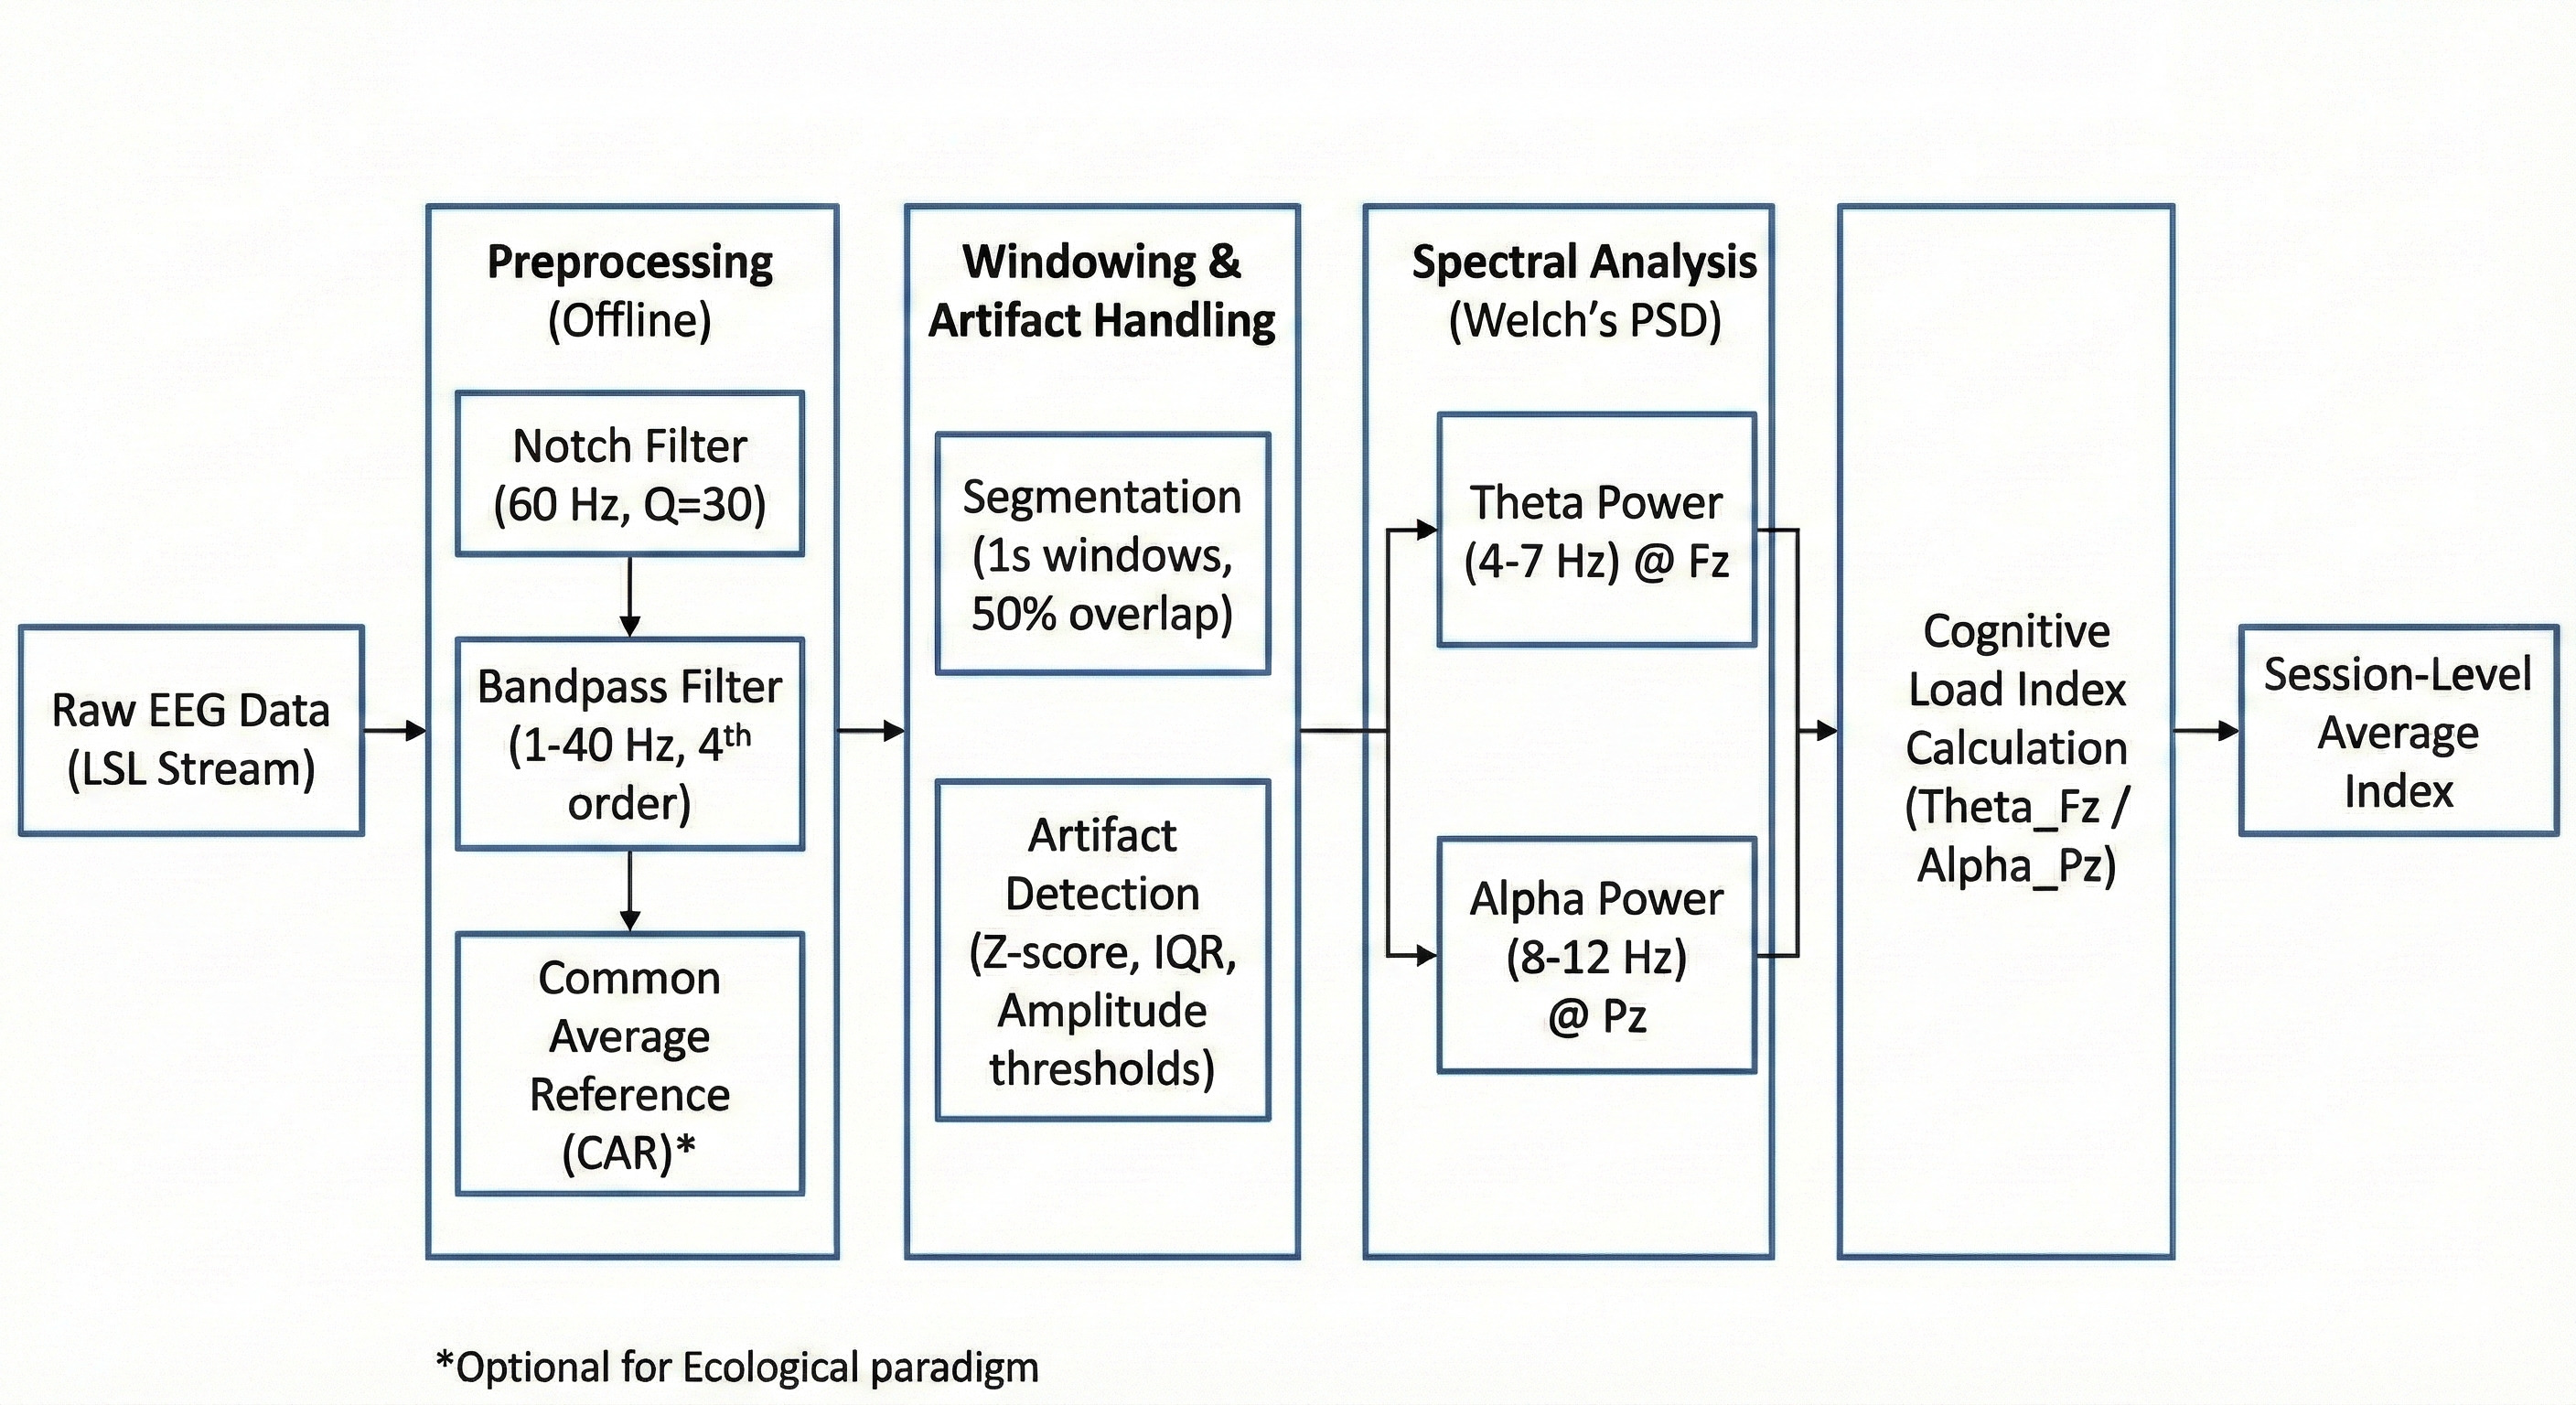
\includegraphics[width=0.9\linewidth]{figures/pipeline1.jpg} 
    \caption{Overview of the EEG processing pipeline and cognitive load index computation. The pipeline includes preprocessing, artifact handling, spectral feature extraction (theta at Fz, alpha at Pz), and index calculation. The asterisk (*) notes steps specific to the ecological paradigm.}
    \label{fig:pipeline}
\end{figure}

\subsection{Artifact detection and window selection}
Artifacts were detected independently for channels Fz and Pz using three criteria: Z-score threshold (3), interquartile range (IQR) threshold (multiplier of 3), and absolute amplitude threshold (200~$\mu$V). Artifact-contaminated samples were handled using linear interpolation to preserve temporal continuity when sufficient surrounding data were available; segments with excessive contamination were excluded from analysis.

After artifact handling, the cognitive load index was recomputed. Only windows with finite index values within a predefined range (0.01--100) were retained. A minimum of two valid windows per phase was required to compute session-level averages, ensuring that estimates reflected more than isolated spectral events.

In some sessions, strict artifact rejection resulted in a limited number of valid analysis windows. This reflects the conservative nature of the predefined signal-quality criteria, particularly under conditions of frontal or parietal contamination. Because the objective of this study was to evaluate session-level trends and discriminative directionality of the index rather than window-level inference, sessions with a minimum of two valid windows were retained to avoid discarding usable recordings while preserving methodological transparency.


\subsection{Controlled paradigm: low vs.\ high cognitive load}
The controlled paradigm followed a baseline--low--high protocol. After a signal verification phase, participants completed a baseline consisting of 90~s with eyes open followed by 90~s with eyes closed. The low cognitive load condition consisted of passive reading for approximately 3~minutes. The high cognitive load condition consisted of a Stroop color--word interference task of similar duration, in which participants identified the ink color rather than the written word using keyboard inputs (R/B/G/Y).

A session was considered \emph{includable} if, in both low and high load phases, the artifact percentage in either Fz or Pz did not exceed 50\% and at least two valid analysis windows remained after cleaning. Among includable sessions, the hypothesis tested was that the mean cognitive load index would be higher in the high-demand condition than in the low-demand condition (High $>$ Low).

\subsection{Subjective cognitive load assessment: NASA-TLX}
Subjective cognitive workload was assessed using the NASA Task Load Index (NASA-TLX), a multidimensional questionnaire capturing Mental Demand, Physical Demand, Temporal Demand, Performance, Effort, and Frustration. Raw (unweighted) NASA-TLX scores were computed and reported as percentages (0--100).

For the controlled paradigm, NASA-TLX was collected as a single global score per participant reflecting the overall session. Consequently, NASA-TLX was not used for within-session Low vs.\ High comparisons. For the ecological paradigm, NASA-TLX scores were collected after task completion for each interaction modality when available and were used descriptively to contextualize perceived workload.

\subsection{Ecological paradigm: exergaming task}
The ecological paradigm involved an interactive exergaming scenario implemented on the platform described in Section~III, supporting keyboard, gamepad, and haptic interaction modalities. Data files did not include explicit low/high phase labels; instead, task segments were identified using event markers and segmented into pre-task and task periods.

Baseline values were obtained from within-session baselines when available; otherwise, from the same participant’s baseline recorded in the controlled paradigm to reduce inter-individual variability.

\begin{equation}
\mathrm{Index}_{\mathrm{norm}} = \frac{\mathrm{Index}_{\mathrm{task}}}{\mathrm{Index}_{\mathrm{baseline}}},
\label{CLI}
\end{equation}

normalized values greater than 1 indicate higher cognitive load during the task compared to baseline.

\subsection{Statistical analysis}
For the controlled paradigm, index values were averaged per session within the low and high cognitive load phases. Group-level descriptive statistics (mean and standard deviation) were computed across includable sessions. Effect size was quantified using paired Cohen’s $d$ computed on session-wise differences (High minus Low).

Given the modest number of includable controlled sessions and conservative artifact rejection, we emphasize descriptive statistics, directionality, and paired effect size (Cohen's $d$) rather than inferential $p$-values.


%%%%%%%%%%%%%%%%%%%%%%%%%%%%%%%%%%%%%%%%%%%%%%%%%%%%%%%%%%%%%%%%%%%%%%%%%%

\section{Results}

\subsection{Controlled paradigm: low vs.\ high cognitive load}

From a total of 14 recorded sessions, six satisfied the predefined signal-quality inclusion criteria (artifact percentage in Fz or Pz $\leq$ 50\% and at least two valid windows after cleaning in both Low and High phases). These includable sessions were used for the primary controlled analysis. At the session level, all included cases exhibited higher mean Theta/Alpha ratios in the high-demand condition (Stroop interference) than in the low-demand condition (passive reading), consistent with the study hypothesis (High $>$ Low).

Table~\ref{tab:controlled} reports per-session mean Theta/Alpha (Fz/Pz) ratios for Low and High conditions, the number of valid analysis windows retained after artifact handling, and the maximum artifact percentage across Fz and Pz in each condition. Despite marked inter-session variability in absolute ratio values and the limited number of valid windows in some sessions, the direction of change (High $>$ Low) was consistent across all included sessions.

\begin{table*}[tbp]
\centering
\caption{\raggedright Per-session summary for the controlled paradigm: mean Theta/Alpha (Fz/Pz) ratio in Low and High Load, valid windows after cleaning, and maximum artifact percentage (Fz or Pz) in each condition.}
\label{tab:controlled}
\footnotesize
\setlength{\tabcolsep}{8pt}
\begin{tabular}{c c c c c}
\toprule
\textbf{Session} & \textbf{Mean Low} & \textbf{Mean High} & \textbf{Valid win (L/H)} & \textbf{Max art.\ \% (L/H)} \\
\midrule
S1 & 3.94 & 6.69  & 2 / 2   & 2.57 / 2.14 \\
S2 & 0.09 & 0.10  & 2 / 2   & 2.36 / 1.06 \\
S3 & 0.30 & 11.36 & 2 / 2   & 2.96 / 26.51 \\
S4 & 0.10 & 0.43  & 59 / 64 & 16.46 / 10.07 \\
S5 & 0.35 & 0.39  & 2 / 2   & 1.92 / 29.15 \\
S6 & 3.42 & 8.97  & 2 / 2   & 7.04 / 4.03 \\
\bottomrule
\end{tabular}
\end{table*}

Sessions with a limited number of valid windows are reported explicitly to ensure transparency and should be interpreted as conservative estimates of session-level index behavior.

At the group level, the mean Theta/Alpha ratio increased from 1.37 (SD = 1.80) during Low Load to 4.65 (SD = 4.99) during High Load, yielding a mean difference (High $-$ Low) of 3.29. The corresponding paired Cohen’s $d$, computed on session-wise differences, was 0.75, indicating a medium effect size. Fig.~\ref{fig:paired_slope} illustrates the Low vs.\ High comparison for each included session.

\begin{figure}[H]
\centering
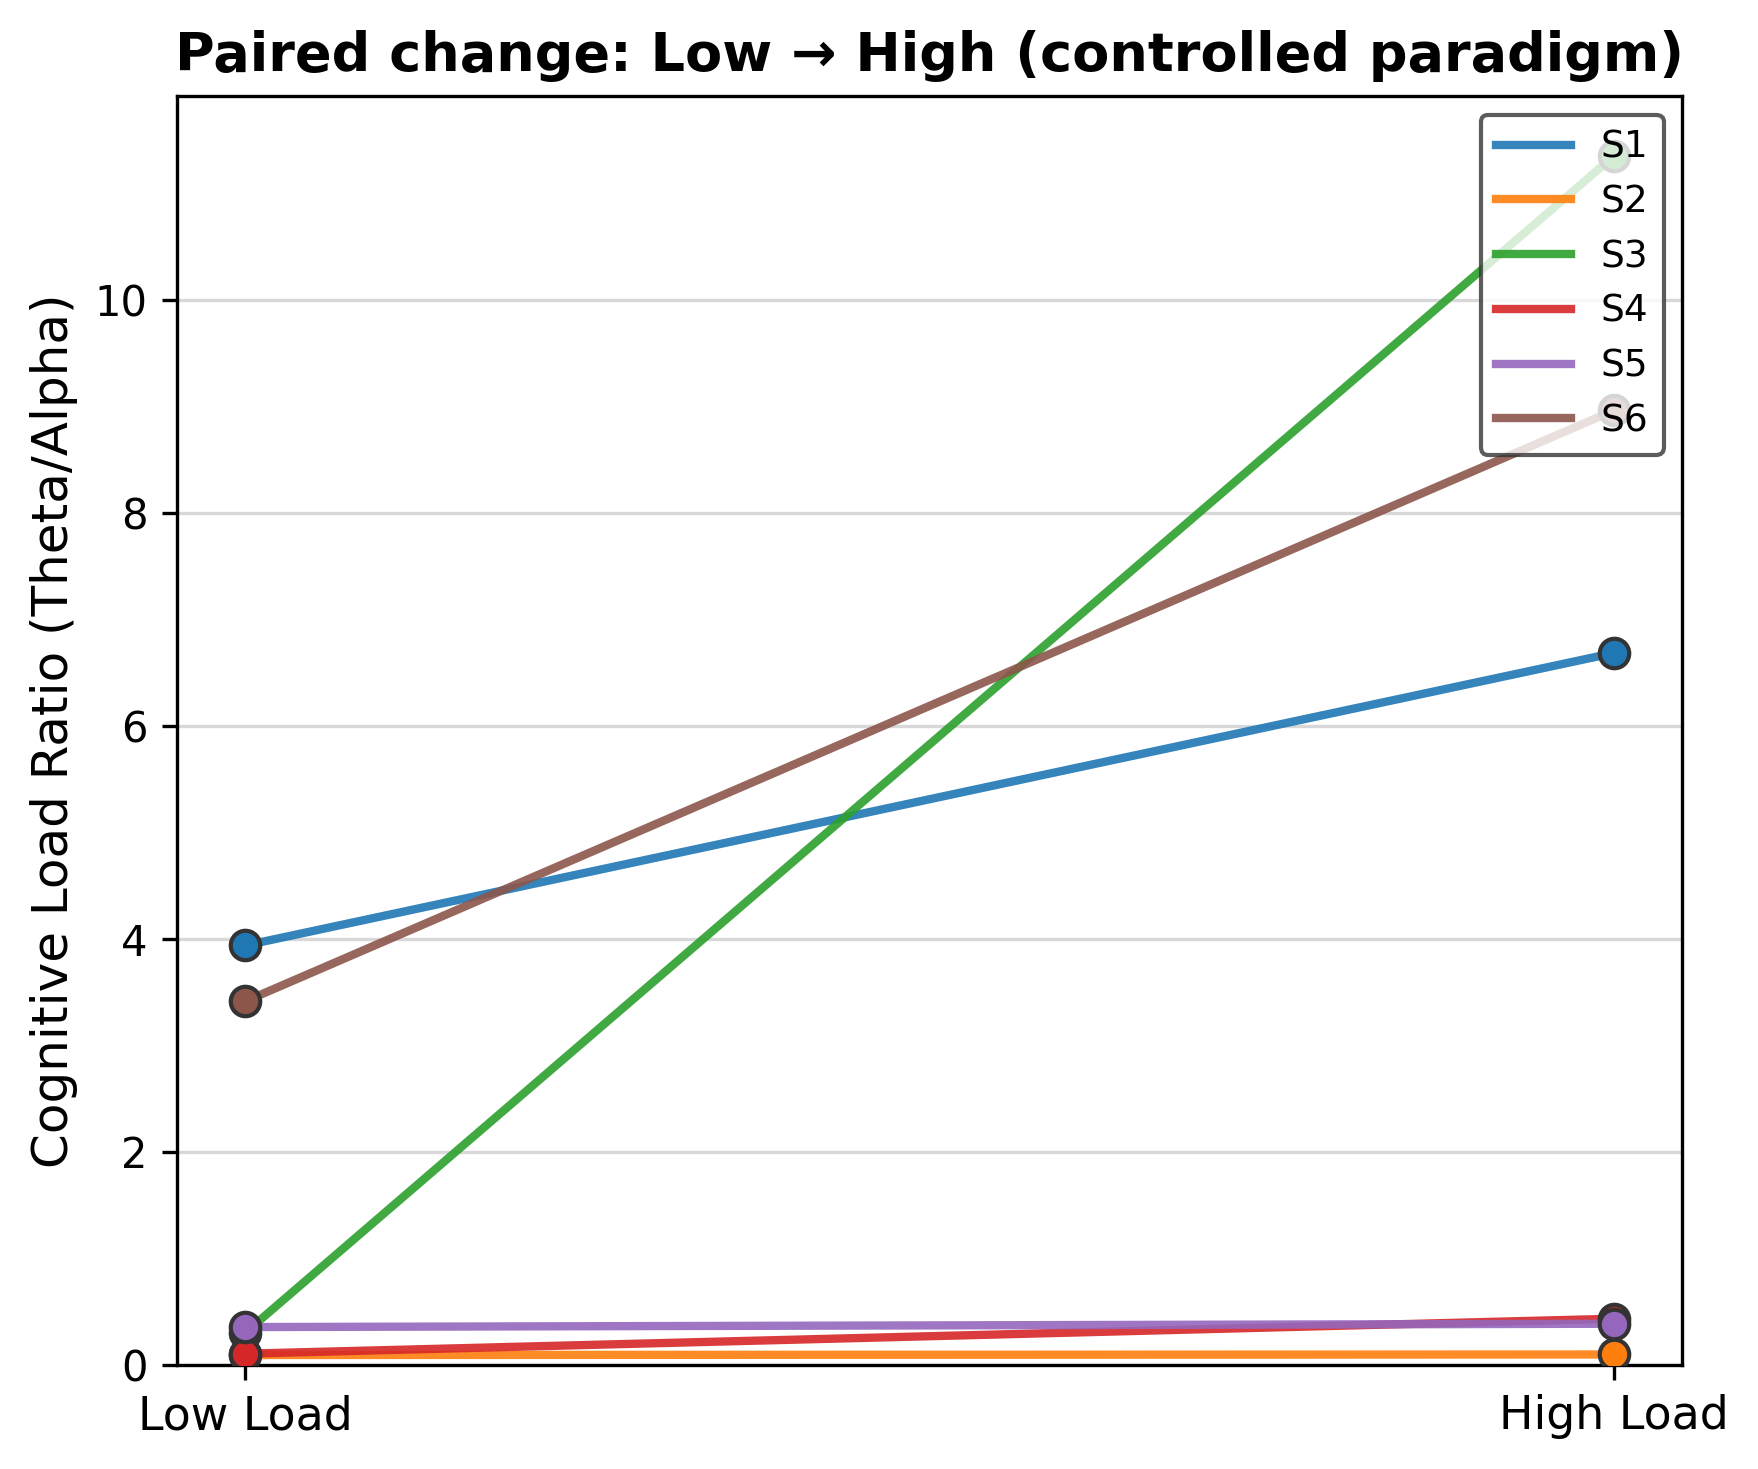
\includegraphics[width=0.7\linewidth]{figures/cumplen_incluibles_paired_slope.png}
\caption{Paired slope plot: Theta/Alpha (Fz/Pz) ratio for each of the six includable sessions from Low Load to High Load (controlled paradigm). Each line represents one session; all lines show an increase, consistent with the hypothesis.}
\label{fig:paired_slope}
\end{figure}

\subsection{Ecological paradigm: exergaming task (baseline-normalized)}

For the ecological exergaming paradigm, analysis was conducted at the session level using recordings that contained an identifiable task segment suitable for baseline comparison. The Theta/Alpha ratio was computed using the same index definition (Fz/Pz) and normalized relative to each session’s baseline value (Equation \ref{CLI}).

%\[
%\mathrm{Index}_{\mathrm{norm}} = \frac{\mathrm{Index}_{\mathrm{task}}}{\mathrm{Index}_{\mathrm{baseline}}}.
%\]
Normalized values greater than 1 indicate higher index values during the task segment relative to baseline.

Across eight analyzed sessions, six exhibited $\mathrm{Index}_{\mathrm{norm}} > 1$ (task $>$ baseline), while two sessions showed $\mathrm{Index}_{\mathrm{norm}} < 1$ (task $<$ baseline). Sessions with $\mathrm{Index}_{\mathrm{norm}} > 1$ yielded normalized ratios of 7.85, 1.87, 2.51, 3.14, 4.08, and 2.14, whereas the remaining two sessions yielded normalized ratios of 0.71 and 0.33.

Figure~\ref{fig:eco_norm} summarizes the baseline-normalized Theta/Alpha (Fz/Pz) ratio for each ecological session. Session identifiers (S1--S8) correspond to recording sessions and do not necessarily represent unique participants, as some participants completed multiple sessions using different interaction modalities. Values above unity indicate increased cognitive load during task execution relative to baseline, whereas values below unity are reported without overinterpretation and may reflect individual differences, baseline selection, or variability in task engagement.

\begin{figure}[H]
    \centering
    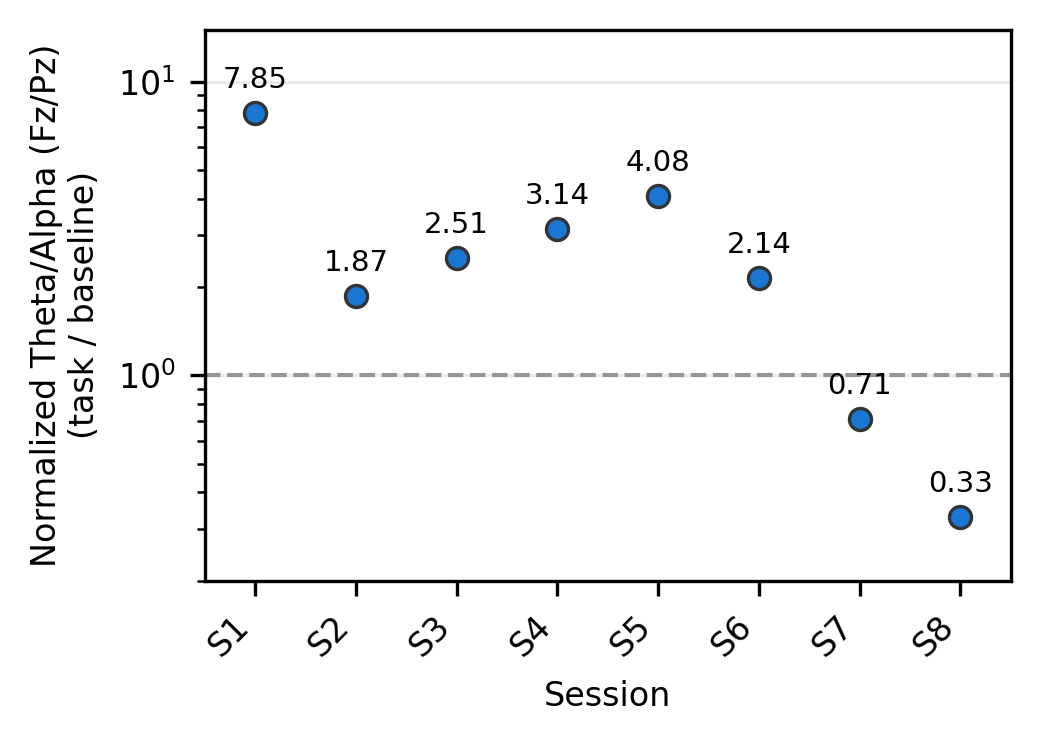
\includegraphics[width=\linewidth]{figures/eco_normalized_ratio_log.png}
    \caption{Ecological paradigm: baseline-normalized Theta/Alpha (Fz/Pz) ratio during the task segment (task/baseline). The dashed line indicates the unity reference (no change relative to baseline).}
    \label{fig:eco_norm}
\end{figure}

\subsection{Subjective workload results}

NASA-TLX scores were used to provide complementary subjective estimates of perceived workload. For the controlled paradigm, a single global NASA-TLX score was collected per participant for the overall session, yielding a mean workload of 48.8\% (SD = 13.5, $N=10$). Because NASA-TLX was not administered separately for Low and High phases, no within-session subjective comparison was performed.

For the ecological exergaming paradigm, NASA-TLX scores were collected per interaction modality when available. Mean subjective workload values were 41.4\% (SD = 14.1) for the Haptic modality, 35.3\% (SD = 13.8) for the Gamepad modality, and 44.1\% (SD = 15.2) for the Keyboard modality ($N=10$). Among the three modalities, the Gamepad condition exhibited the lowest perceived workload on average.

Overall, NASA-TLX results indicate moderate subjective workload across both paradigms and provide contextual information that complements the EEG-derived cognitive load indices without implying direct correspondence at the session or phase level.
%%%%%%%%%%%%%%%%%%%%%%%%%%%%%%%%%%%%%%%%%%%%%%%%%%%%%%%%%%%%%%%%%%%%%%%%%%%%%%
\section{Discussion}

This study evaluated the Theta/Alpha ratio computed from frontal and parietal EEG channels (Fz/Pz) as an index of cognitive load across two complementary paradigms: a controlled laboratory benchmark and an ecological interactive task. In the controlled setting, the index consistently discriminated between low cognitive load (passive reading) and high cognitive load (Stroop interference) across all includable sessions, yielding a medium effect size at the group level. These findings support the Theta/Alpha (Fz/Pz) ratio as a compact and interpretable marker of cognitive demand under well-defined experimental conditions, consistent with prior work linking frontal theta increases and parietal alpha modulation to mental workload~\cite{c1,c3,c7}.

The increase in the Theta/Alpha ratio observed during the Stroop task aligns with established neurophysiological interpretations of frontal theta as a marker of executive control and conflict monitoring, together with parietal alpha suppression reflecting increased task engagement. Comparable spectral patterns have been reported in previous EEG studies using Stroop and related interference paradigms, reinforcing the suitability of this task as a benchmark for workload validation~\cite{c5,c9}. Importantly, the present results were obtained using a predefined and explicitly reported preprocessing and artifact-handling pipeline, addressing methodological concerns regarding the reproducibility and stability of EEG-based workload indices highlighted in recent literature~\cite{c4,c6}. Such transparency is essential when proposing user-state metrics intended for integration into intelligent systems.

Beyond controlled validation, the ecological exergaming paradigm provided a structured yet interactive context for examining the behavior of the same index under less constrained conditions. In the majority of analyzed sessions, baseline-normalized Theta/Alpha ratios increased during task execution, indicating sensitivity to cognitive demand associated with sustained attention and sensorimotor interaction. These observations are consistent with reports of EEG workload modulation in immersive and game-based environments, where task demands and engagement fluctuate dynamically~\cite{c2,c3}. At the same time, notable inter-session variability was observed, with a subset of sessions exhibiting normalized ratios below unity.

Such variability is expected in ecological paradigms and may reflect differences in baseline selection, individual engagement strategies, learning effects, or interaction modality. For real-world human--machine systems, this variability underscores the importance of normalization strategies and session-level trend analysis rather than strict threshold-based interpretations. In this context, the present findings support the sensitivity—but not uniform monotonicity—of the Theta/Alpha ratio when applied to interactive scenarios.

Subjective workload, assessed using NASA-TLX, provided complementary context for interpreting task demand. Because NASA-TLX was not administered at the same temporal or phase resolution as the EEG analysis, these subjective measures were not used for direct correlation or inferential validation of the EEG index. Instead, they serve to contextualize perceived task demand alongside objective neurophysiological measures.

Several limitations should be acknowledged. First, the number of includable sessions in the controlled paradigm was constrained by strict signal-quality criteria, resulting in a modest sample size and, in some cases, a limited number of valid analysis windows. Second, ecological analyses were conducted at the session level without applying identical exclusion thresholds, precluding direct statistical comparison between paradigms. Finally, short analysis windows, while appropriate for capturing temporal dynamics, may increase variance in spectral estimates when data availability is limited.

Future work will focus on expanding the dataset, incorporating graded task difficulty levels, and examining real-time implementations of the Theta/Alpha (Fz/Pz) index for workload-aware intelligent systems. Integrating this metric into adaptive human--machine interaction architectures represents a promising direction for bridging controlled validation with applied operational environments~\cite{c10}.
%%%%%%%%%%%%%%%%%%%%%%%%%%%%%%%%%%%%%%%%%%%%%%%%%%%%%%%%%%%%%%%%%%%%%%%%%%%%

%%%%%%%%%%%%%%%%%%%%%%%%%%%%%%%%%%%%%%%%%%%%%%%%%%%%%%%%% INICIO SECCIÓN:
% APORTACIÓN DE JERÓNIMO APARICIO-JUÁREZ
%%%%%%%%%%%%%%%%%%%%%%%%%%%%%%%%%%%%%%%%%%%%%%%%%%%%%%%%%
\section{Colaboración de Jerónimo}



\subsection{Arquitectura de la plataforma de exergaming y protocolo de interacción.}

Esta sección describe la arquitectura técnica y el diseño experimental de la plataforma \textit{ADHD K9 CanineQuest}, la cual ha sido desarrollada específicamente para la estimulación y evaluación de procesos neurocognitivos en niños con TDAH. El sistema integra hardware de interacción avanzada y entornos virtuales con el objetivo de determinar los niveles de concentración visual y procesamiento cognitivo del usuario durante la ejecución de tareas motrices coordinadas.

\subsubsection{Gestión de estados y lógica de control.}

El flujo operativo del exergame se rige por una máquina de estados finitos (FSM), la cual garantiza el determinismo durante las transiciones experimentales. La FSM coordina la sincronización entre los estímulos visuales y los protocolos de adquisición de datos en tres etapas principales: reposo (\textit{baseline}), guiado pasivo y exploración activa. Esta estructura permite aislar y medir de forma precisa la demanda de procesamiento visual y mental asociada a cada paradigma de interacción.

%\begin{figure}[H]
%    \centering
%    \includegraphics[width=\linewidth, keepaspectratio]{figures/FSM_diagram.png} 
%    \caption{Máquina de estados finitos (FSM) del exergame.}
%    \label{fig:fsm_logica}
% \end{figure}

\subsubsection{Interfaces multimodales y dinámica de interacción.}

Se implementaron tres modalidades de entrada para evaluar la variabilidad del control motor y su relación con la carga cognitiva: teclado, mando de juego (\textit{gamepad}) y un dispositivo háptico de eslabones articulados. En la modalidad háptica, el sistema permite la renderización de fuerzas constantes y de resorte, proporcionando una retroalimentación cinestésica que incrementa la demanda de coordinación sensorio-motora, facilitando la observación de fluctuaciones en la concentración mental.

\subsubsection{Paradigma de exploración activa.}

En el modo de exploración activa, el usuario ejerce el control total sobre la trayectoria espacial. Desde la perspectiva del control de movimiento, el sistema opera como un lazo abierto, capturando la intención motriz y el procesamiento visual proactivo del sujeto. El vector de estado cinemático $\mathbf{P} = [x, y, z]^T$ y el vector de fuerzas dinámicas $\mathbf{F} = [F_x, F_y, F_z]^T$ se registran en tiempo real para correlacionar la precisión del movimiento con el estado cognitivo.

\begin{figure*}[htbp]
   \centering
   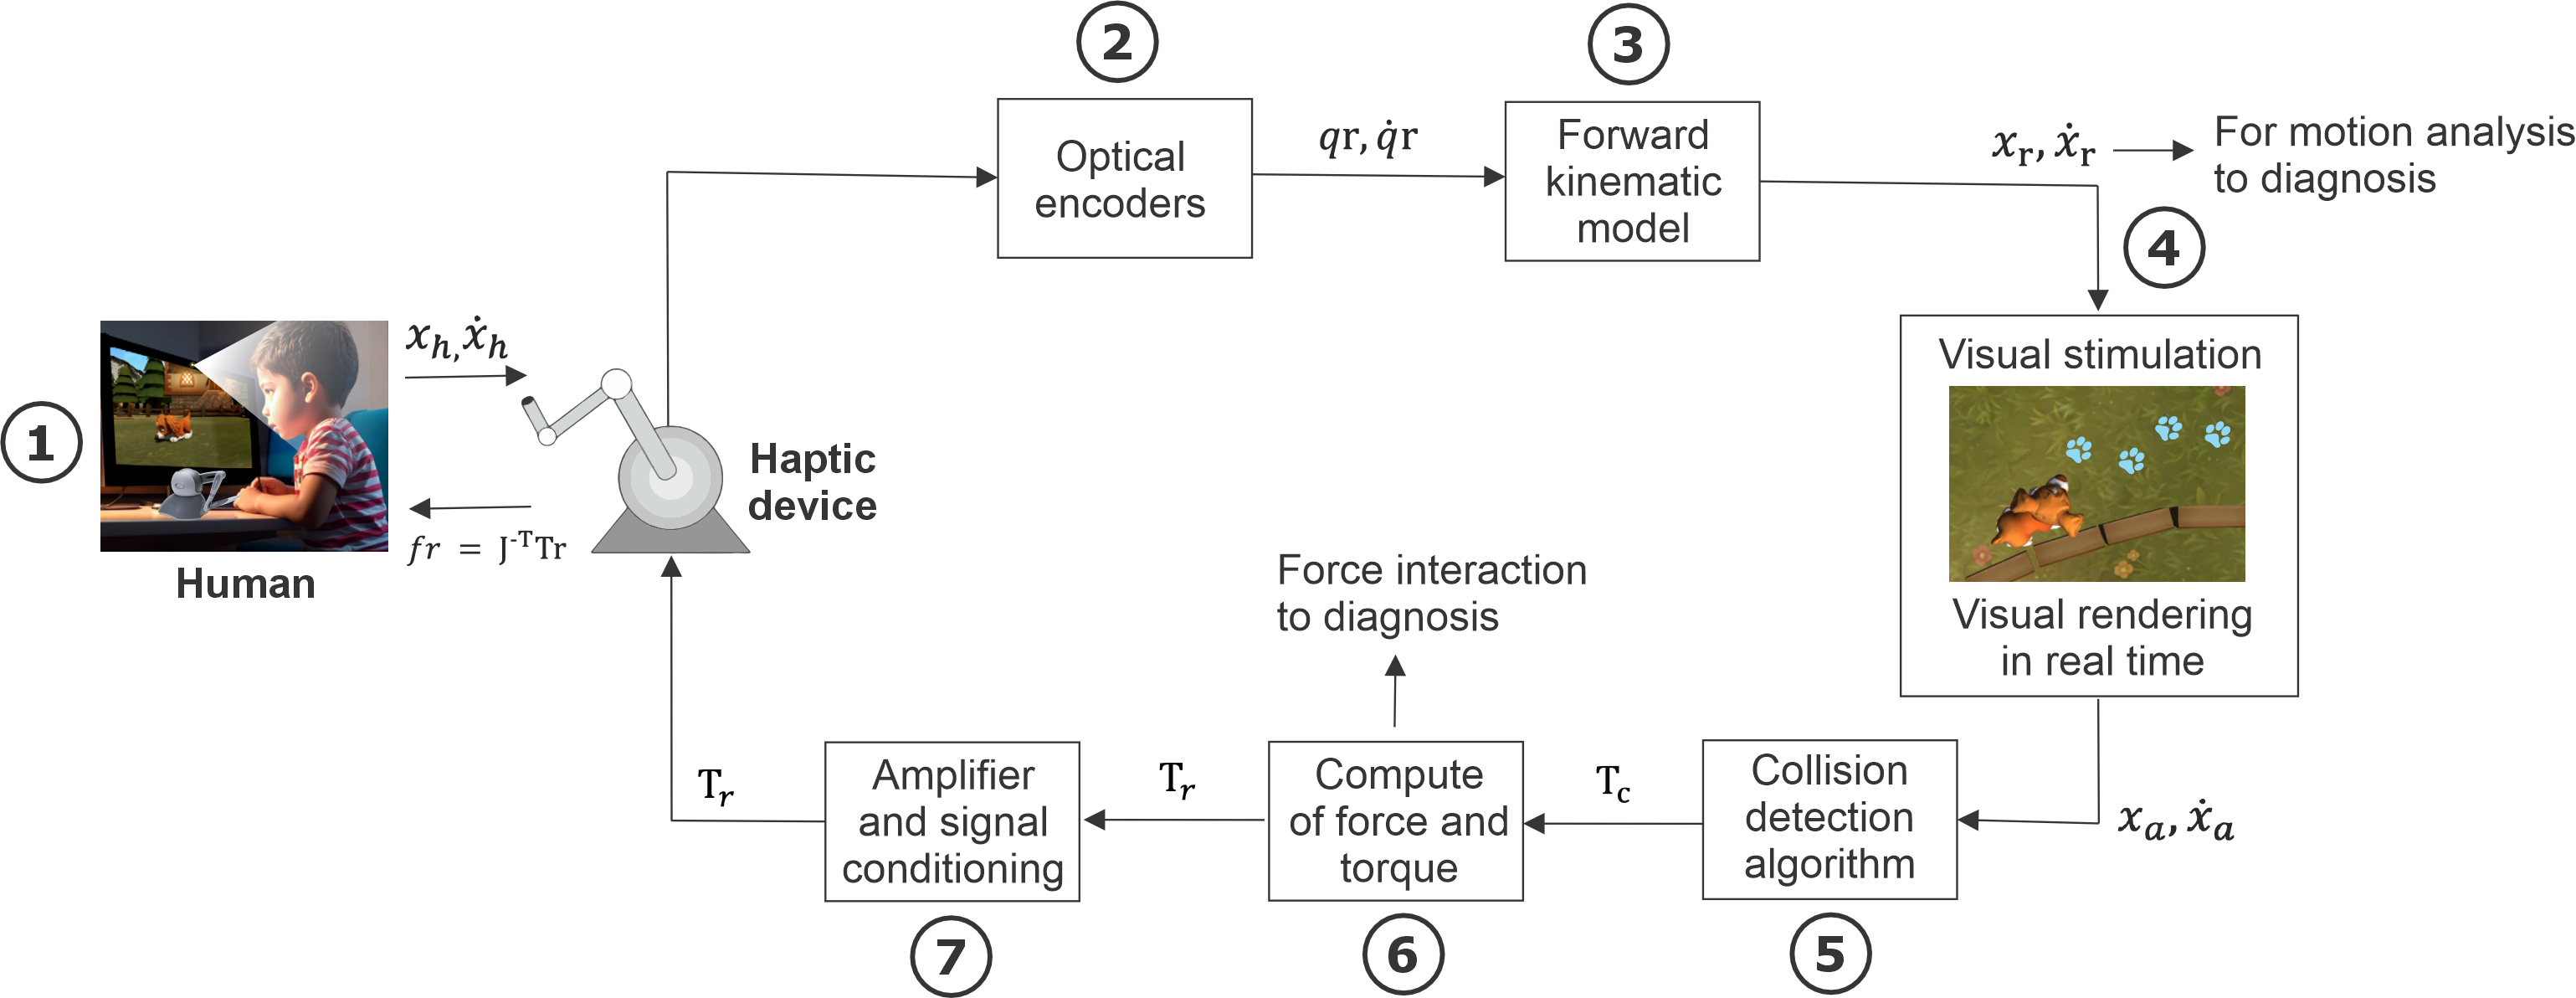
\includegraphics[width=1\linewidth]{figures/ActiveHapticExploration_EN.png}
   \caption{Diagrama de bloques del lazo de control en modo de exploración activa.}
   \label{ActiveHapticExploration_EN}
\end{figure*}




\subsubsection{Adquisición de métricas y conjunto de datos de desempeño.}

La plataforma genera un conjunto de datos (\textit{dataset}) con una tasa de actualización de 0.01 s, diseñado para cuantificar el desempeño técnico y cognitivo. Las métricas incluyen variables temporales para evaluar la persistencia atencional, coordenadas espaciales para el análisis de trayectoria y magnitudes de fuerza. Estos indicadores constituyen el fundamento técnico para validar el índice de carga cognitiva y la capacidad de concentración visual y mental del usuario durante la tarea.


%%%%%%%%%%%%%%%%%%%%%%%%%%%%%%%%%%%%%%%%%%%%%%%%%%%%%%%%%%%%%%%%%%%%%%%%%%%%% SECCION IA DEFINIR SI INTEGRAR O NO
\section{Artificial Intelligence Pipeline and Modeling}

To complement the neurophysiological analysis, an artificial intelligence (AI) pipeline was developed to process EEG recordings and evaluate their suitability for cognitive load classification. The study employed a publicly available EEG dataset containing recordings acquired during Arithmetic and Stroop tasks, designed for cognitive workload analysis \cite{Nirabi2025_EEGDataset}.

\subsection{Dataset and data organization}

The dataset consists of multi-channel EEG recordings collected under controlled experimental conditions, including baseline, arithmetic tasks, and Stroop interference tasks. The signals were originally stored in raw text format and subsequently converted into structured CSV files for processing.

Each recording was organized into:
(i) sample-level data, representing continuous EEG signals, and  
(ii) window-level data, obtained through temporal segmentation.

\subsection{Preprocessing and feature extraction}

EEG signals were segmented into windows of 4 seconds with 50\% overlap, corresponding to 1000 samples per window at a sampling rate of 250 Hz. Prior to feature extraction, each window and channel underwent a preprocessing pipeline to improve signal quality and spectral consistency.

The preprocessing steps included:

\begin{itemize}
\item Band-pass filtering (1--40 Hz) using a 4th-order Butterworth filter
\item Linear detrending to remove DC components and slow drift
\item Notch filtering at 50 Hz and 60 Hz to attenuate power line noise
\end{itemize}

These operations were applied using zero-phase filtering to avoid phase distortion. Feature extraction was then performed on the preprocessed signals.

Each window was represented through a combination of time-domain and frequency-domain features. Time-domain descriptors included mean, standard deviation, minimum, maximum, root mean square (RMS), and mean absolute value.

Frequency-domain features were computed using Welch's method, extracting band power values for delta, theta, alpha, beta, and gamma bands. In addition, relative band powers were calculated to normalize spectral contributions across channels.

To capture cross-frequency relationships, band ratios such as theta/alpha and beta/alpha were included. Spectral entropy was also computed as a measure of signal complexity within the 1--40 Hz range.

\subsection{Training protocol}

To ensure a realistic evaluation, the dataset was split at the file level rather than at the window level. This prevents data leakage between training and testing sets, as multiple windows originating from the same recording are not distributed across both sets.

Class imbalance was addressed using Synthetic Minority Over-sampling Technique (SMOTE) applied only to the training set. Additionally, class weights were incorporated during model training to improve the detection of minority classes, particularly the baseline (normal) condition.

\subsection{Results and analysis}

The three-class classification problem (low, normal, high) showed limited separability, particularly for the low-load condition. Models consistently failed to identify this class, indicating that EEG patterns corresponding to intermediate cognitive load levels overlap significantly in the feature space.

In contrast, the binary classification problem (baseline vs task-related activity) produced more stable and meaningful results. Random Forest achieved the best overall performance, reaching approximately 78--80\% accuracy.

However, a more detailed analysis revealed an asymmetric performance across classes. The model achieved high recall for the task-related condition (above 90\%), while the recall for the baseline condition remained around 40\%. This indicates that the classifier is more sensitive to detecting cognitive engagement than to identifying resting states.

\subsection{Discussion}

The results suggest that EEG signals, when analyzed using short temporal windows, are more effective for distinguishing between resting and task-engaged states than for resolving fine-grained differences in cognitive load.

The difficulty in separating low and high cognitive load conditions highlights the intrinsic overlap of EEG patterns across intermediate task demands. This limitation is likely related to both the short window duration and the variability of cognitive strategies across subjects.

From a modeling perspective, classical machine learning approaches based on engineered spectral features outperformed the CNN+LSTM architecture under the current dataset conditions. This suggests that feature-based representations remain a robust and practical solution for EEG classification when data availability is limited.

Overall, the findings support the formulation of cognitive load estimation as a binary discrimination problem in practical applications, while also identifying key challenges for extending these approaches to multi-level workload classification.

\begin{figure}[H]
\centering
\resizebox{\columnwidth}{!}{%
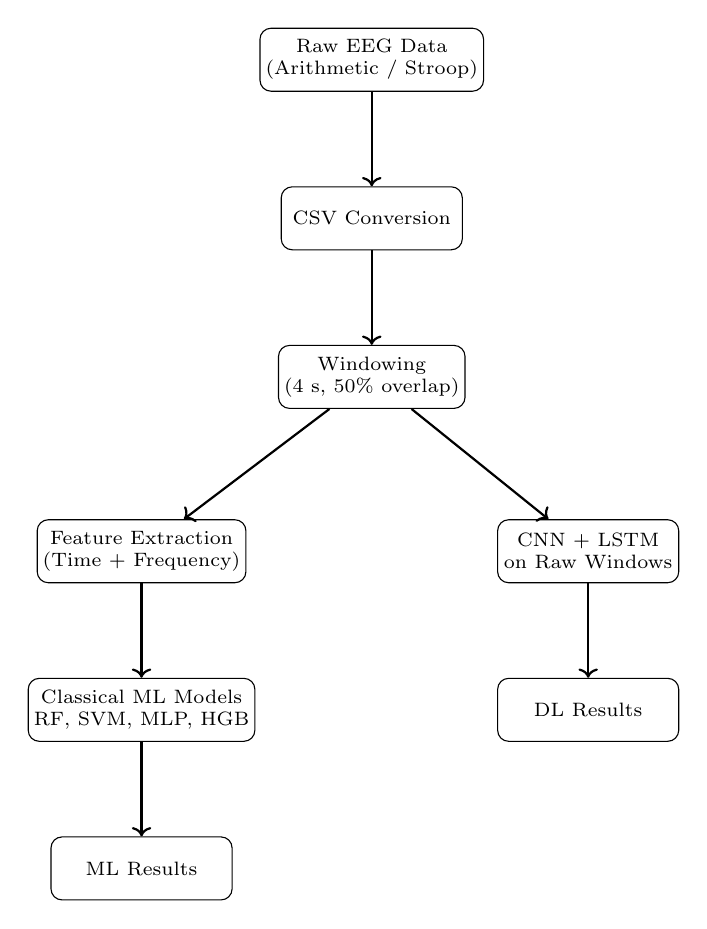
\begin{tikzpicture}[
node distance=1.2cm and 0.5cm,
every node/.style={
draw,
rectangle,
rounded corners,
align=center,
minimum width=2.3cm,
minimum height=0.8cm,
font=\scriptsize,
inner sep=2pt
},
arrow/.style={->, thick}
]

\node (raw) {Raw EEG Data\\(Arithmetic / Stroop)};
\node (csv) [below=of raw] {CSV Conversion};
\node (window) [below=of csv] {Windowing\\(4 s, 50\% overlap)};

\node (features) [below left=1.4cm and 0.4cm of window] {Feature Extraction\\(Time + Frequency)};
\node (dl) [below right=1.4cm and 0.4cm of window] {CNN + LSTM\\on Raw Windows};

\node (ml) [below=of features] {Classical ML Models\\RF, SVM, MLP, HGB};
\node (outdl) [below=of dl] {DL Results};
\node (outml) [below=of ml] {ML Results};

\draw[arrow] (raw) -- (csv);
\draw[arrow] (csv) -- (window);

\draw[arrow] (window) -- (features);
\draw[arrow] (window) -- (dl);

\draw[arrow] (features) -- (ml);
\draw[arrow] (ml) -- (outml);

\draw[arrow] (dl) -- (outdl);

\end{tikzpicture}%
}
\caption{One-column schematic of the proposed AI pipeline. Classical machine learning models were trained on engineered features extracted from windowed EEG segments, whereas the CNN+LSTM branch operated directly on raw EEG windows.}
\label{fig:pipeline}
\end{figure}


\begin{figure}[H]
\centering
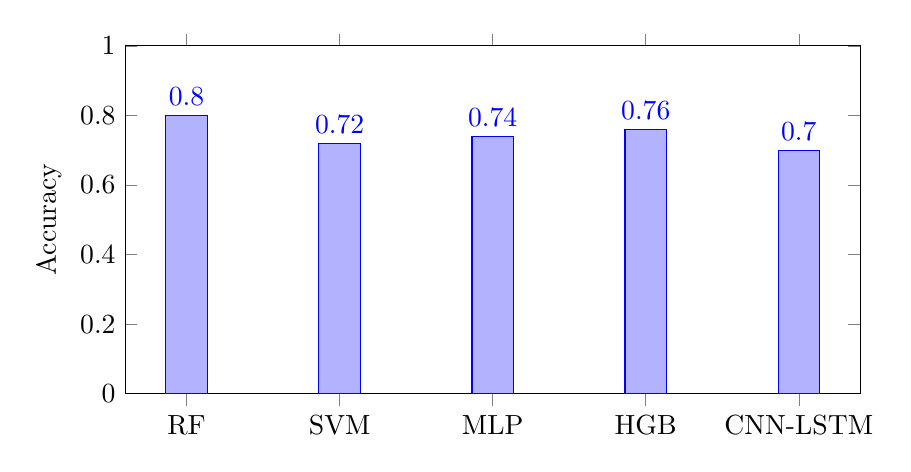
\begin{tikzpicture}
\begin{axis}[
ybar,
bar width=15pt,
width=0.9\linewidth,
height=6cm,
ylabel={Accuracy},
symbolic x coords={RF,SVM,MLP,HGB,CNN-LSTM},
xtick=data,
ymin=0, ymax=1,
nodes near coords,
]

\addplot coordinates {
(RF,0.80)
(SVM,0.72)
(MLP,0.74)
(HGB,0.76)
(CNN-LSTM,0.70)
};

\end{axis}
\end{tikzpicture}
\caption{Comparison of classification accuracy across evaluated models in the binary scenario.}
\label{fig:results}
\end{figure}
%%%%%%%%%%%%%%%%%%%%%%%%%%%%%%%%%%%%%%%%%%%%%%%%%%%%%%%%%%%%%%%%%%%%%%%%%%%%%
\section{Conclusion}

This study validated the Theta/Alpha ratio computed from frontal and parietal EEG channels (Fz/Pz) as a practical and interpretable index of cognitive load across controlled and ecological contexts. Under a controlled baseline--low--high protocol, the index reliably discriminated passive reading from Stroop interference in six sessions satisfying predefined signal-quality criteria. The increase from 1.37 (SD = 1.80) to 4.65 (SD = 4.99), together with a paired Cohen’s $d = 0.75$, supports the discriminative validity of the Theta/Alpha (Fz/Pz) ratio under well-defined laboratory conditions.

Beyond controlled validation, the same index exhibited sensitivity to task engagement in an ecological interactive scenario. Baseline-normalized Theta/Alpha ratios increased in the majority of analyzed sessions, while also revealing inter-session variability characteristic of naturalistic human--machine interaction contexts. These results indicate that the proposed index can capture cognitive load dynamics beyond strictly scripted tasks when appropriate normalization and session-level analysis are applied.

Overall, the findings support the Theta/Alpha (Fz/Pz) ratio as a compact and implementation-ready EEG-based metric for cognitive load estimation in workload-aware human--machine systems. This dual validation establishes a methodological foundation for future real-time and adaptive user-state estimation frameworks in intelligent interaction environments.

\section*{Acknowledgment}
The authors thank the Mirai Innovation Research Institute for providing the experimental infrastructure and technical support, including the AURA EEG acquisition system used in this study. The Advanced Robotics and Haptic Interfaces Laboratory (UAEH) is also acknowledged for the development and maintenance of the interactive exergaming platform employed in the ecological paradigm.

E. R. Hernandez-Rios and J. Aparicio-Juarez acknowledge the Secretariat of Science, Humanities, Technology and Innovation (SECIHTI), Mexico, for the doctoral scholarships received. O. A. Dominguez-Ramirez acknowledges support from the National System of Researchers (SNII), SECIHTI, Mexico.


\section*{conflict of interest}
The authors declare no conflict of interest.

\section*{References}

\begin{thebibliography}{99}
\footnotesize


\bibitem{c1}
B. Raufi and L. Longo, ``An Evaluation of the EEG alpha-to-Theta and Theta-to-alpha Band Ratios as Indexes of Mental Workload,'' \emph{Front. Neuroinform.}, vol. 16, p. 861967, 2022. doi:10.3389/fninf.2022.861967

\bibitem{c2}
R. Khan et al., ``Assessing cognitive load using EEG and eye-tracking in immersive environments,'' \emph{Multimodal Technol. Interact.}, vol. 9, no. 9, p. 99, 2025. doi:10.3390/mti9090099

\bibitem{c3}
A. D. Blanco et al., ``EEG spectral power correlates across cognitive tasks with Theta-to-alpha Ratio (TAR) significance,'' \emph{J. Neurosci. Methods}, vol. 410, p. 110292, 2025. doi:10.1016/j.biopsycho.2025.109084

\bibitem{c4}
S. Chikhi, N. Matton, and S. Blanchet, ``EEG power spectral measures of cognitive workload: A meta-analysis,'' \emph{Psychophysiology}, vol. 59, no. 6, p. e14009, 2022. doi:10.1111/psyp.14009

\bibitem{c5}
M. Pušica et al., ``Machine learning performance in EEG-based mental workload estimation and frontal midline theta activity,'' \emph{Front. Neuroergon.}, vol. 5, p. 135678, 2025. doi:10.3389/fnrgo.2025.1621309

\bibitem{c6}
M. Mondellini and S. Caggiula, ``A multimodal approach exploiting EEG to investigate mental workload,'' \emph{Int. J. Hum.-Comput. Stud.}, vol. 181, p. 103180, 2024. doi:10.1080/10447318.2023.2258017

\bibitem{c7}
S. Moontaha and A. Mathew, ``Wearable EEG-based cognitive load classification using spectral band ratios,'' \emph{Brain Sci.}, vol. 13, no. 9, p. 1234, 2023. doi: 10.5220/0011628300003414

\bibitem{c8}
E. Khan et al., ``Theta activity and cognitive functioning: Task-related increases in frontal theta during cognitive demand,'' \emph{Cogn. Neurosci.}, vol. 15, no. 1, p. 45-58, 2024. doi:10.1016/j.dcn.2024.101404

\bibitem{c9}
J. Wu et al., ``Brain functional connectivity changes induced by cognitive tasks including Stroop,'' \emph{Sci. Rep.}, vol. 15, p. 4567, 2025. doi:10.1038/s41598-025-08330-6

\bibitem{c10}
A. Arana-De-Las Casas et al., ``Real-time mental workload measurement for cognitive tasks using an EEG-based workload index,'' \emph{bioRxiv (Preprint)}, 2024. doi:10.21203/rs.3.rs-4442355/v1

\bibitem{14}
A. Serrano-Barroso et al., ``Detecting attention levels in ADHD children with a video game,'' \emph{Sensors}, vol. 21, no. 9, p. 3221, 2021. doi:10.3390/s21093221

\bibitem{15}
H. Ji et al., ``The Effects of Exergaming on Attention in Children With ADHD,'' \emph{JMIR Serious Games}, vol. 11, p. e40438, 2023. doi:10.2196/40438

\bibitem{16}
B. Tleubayev et al., ``Robot-assisted therapy for children with ADHD and ASD,'' \emph{ACM ICPS}, pp. 58–62, 2019. doi:10.1145/3325693.3325703

\bibitem{22} 
O. A. Dominguez-Ramirez and V. Parra-Vega, ``Active haptic exploration of deformable objects,'' \emph{DAAAM Int. Scientific Book}, pp. 177–190, 2006.

\bibitem{23} 
O. A. Dominguez-Ramirez and V. Parra-Vega, ``Texture, Roughness and Shape Haptic Perception,'' \emph{Proc. IEEE/RSJ IROS}, 2003. doi:10.1109/IROS.2003.1249634

\bibitem{24}
A. Almukhtar, V. Caddick, R. Naik, M. Goble, G. Mylonas, A. Darzi, 
F. Orihuela-Espina, and D. R. Leff, 
``Objective Assessment of Cognitive Workload in Surgery: A Systematic Review,'' 
\emph{Ann. Surg.}, vol. 281, no. 6, pp. 942--951, Jun. 2025, 
doi: 10.1097/SLA.0000000000006370.

\bibitem{CavanaghFrank2014_FrontalTheta}
J. F. Cavanagh and M. J. Frank,
``Frontal theta as a mechanism for cognitive control,''
\emph{Trends in Cognitive Sciences}, vol. 18, no. 8, pp. 414--421, 2014.
doi:10.1016/j.tics.2014.04.012

\bibitem{Klimesch2007_AlphaInhibitionTiming}
W. Klimesch, P. Sauseng, and S. Hanslmayr,
``EEG alpha oscillations: The inhibition--timing hypothesis,''
\emph{Brain Research Reviews}, vol. 53, no. 1, pp. 63--88, 2007.
doi:10.1016/j.brainresrev.2006.06.003

\bibitem{Mastropietro2023_ReliabilityFzPz}
A. Mastropietro et al.,
``Reliability of mental workload index assessed by EEG with different electrode configurations and signal pre-processing pipelines,''
\emph{Sensors}, vol. 23, no. 3, p. 1367, 2023.
doi:10.3390/s23031367

\bibitem{BigdelyShamlo2015_PREP}
N. Bigdely-Shamlo et al.,
``The PREP pipeline: standardized preprocessing for large-scale EEG analysis,''
\emph{Frontiers in Neuroinformatics}, vol. 9, p. 16, 2015.
doi:10.3389/fninf.2015.00016

\bibitem{DiFlumeri2018_RealDrivingMWL}
G. Di Flumeri et al.,
``EEG-Based Mental Workload Neurometric to Evaluate the Impact of Different Traffic and Road Conditions in Real Driving Settings,''
\emph{Frontiers in Human Neuroscience}, vol. 12, p. 509, 2018.
doi:10.3389/fnhum.2018.00509

\bibitem{Dehais2019_RealFlightDryEEG}
F. Dehais et al.,
``Monitoring Pilot's Mental Workload Using ERPs and Spectral Power with a Six-Dry-Electrode EEG System in Real Flight Conditions,''
\emph{Sensors}, vol. 19, no. 6, p. 1324, 2019.
doi:10.3390/s19061324

\bibitem{Nirabi2025_EEGDataset}
A. Nirabi, F. A. Rahman, M. H. Habaebi, K. A. Sidek, and S. Yusoff,
``Cognitive load assessment through EEG: A dataset from arithmetic and Stroop tasks,''
\emph{Data in Brief}, vol. 60, p. 111477, 2025.
doi:10.1016/j.dib.2025.111477

\end{thebibliography}

\end{document}

